\chapter{Abstract Extended}

\section{Uvod}

Od začátku průmyslové revoluce, složitost
výrobní stroje a sériové linky se postupně zvyšovaly a vyžadují
neustálé sledování podmínek systémů z ekonomických důvodů.
Na druhou stranu kritické systémy jako letadla, kosmické lodě,
automobilové systémy, jaderné reaktory a další vyžadují okamžitý poplach
chyba, lokalizovat došlo k chybě a ještě více předvídat možnou budoucnost
poruchy. Tyto požadavky se staly předpoklady pro detekci chyb
a pole Analýza a Prediktivní údržba.

Výrobní proces vždy zahrnoval prvky kontroly chyb a online
monitorování. Od prvních metod detekce poruch, například vizuální
inspekce, dnešní továrny přecházejí na automatizované systémy skládající se z
senzory a výpočetní jednotky k vyhodnocení poruch. Někdy je
kritické pro sledování zpracovatelského zařízení v reálném čase, aby nedošlo k poškození
způsobené chybou nebo anomálií. Každá jednotlivá chyba může způsobit zpomalení
výrobní proces a tím i snížení zisku.

Algoritmy monitorování zařízení v reálném čase vytvořily Fault Detection a
Pole analýzy (FDA). Metody FDA ve většině případů nevyžadují stroj
techniky učení a dokáže detekovat poruchy pomocí základních algoritmů
od Fourierovy analýzy a algoritmů pro kontrolu trendů po složitější
techniky, jako jsou Gaussovské modely směsí.

Vzhledem k množství údajů shromážděných v posledních letech a rozšíření
technologie ukládání dat jako cloudové služby a efektivita výpočtu, to
je možné používat pokročilejší algoritmy pro detekci poruch a
analýza. Pomocí technik klasifikace strojového učení je to možné
izolovat, kde se chyba vyskytuje. Další možnost, která se stane
k dispozici s velkým množstvím dat je odhad zbývajícího užitečného
život (RUL) celého systému. Tyto techniky vedly k predikci
údržba jako snaha o optimální řešení údržby. Aktuální
technický stav zařízení je vždy k dispozici podle informací
extrahované z měřených signálů. Je možné použít aktuální systém
podmínky pro odhad zbývající životnosti v čase nebo vzdálenosti
měření, jako jsou dny, kilometry nebo cykly. Odhadovaný zbytek
životnost dává možnost plánovat údržbu týkající se skutečného systému
podmínky.

Tyto zbývající algoritmy pro odhad životnosti, detekce poruch
metody a techniky modelování a identifikace systémů tvoří nový
pole prediktivní údržby.

Modelování systému umožňuje poskytovat experimenty a vyvíjet řešení
offline před fyzickými implementacemi hardwaru. Nedostupné nebo
náročné implementovat měření lze nahradit generovanými daty
ze simulačního modelu a nakonec pomáhá nasadit robustní algoritmus.

Tato práce poskytuje krátký úvod do detekce poruch a predikce
metodiky údržby a základní terminologie.
Kapitola \ref{ch: teor_surv} popisuje hlavní cíl a problémy
v těchto oblastech a zaměřuje se na podobnosti a rozdíly mezi nimi
dva přístupy.

Vývoj simulačního modelu dvojčinného pneumatického aktuátoru a
porovnání s reálným vybavením pomocí různých přístupů je
popsané v kapitolách 3, 4 a 5.

Následující kapitola 6 ilustruje prediktivní údržbu založenou na signálu
metody využívající různé senzory dostupné v demonstračním zařízení.
Aplikování předzpracování, extrakce funkcí a klasifikační model,
senzory byly hodnoceny z hlediska funkčnosti, přesnosti a ceny.

Techniky prediktivní údržby založené na modelu a simulační model
využití je demonstrováno v kapitole 7. Simulační model je zvyklý
určit zbytkové signály mezi naměřenými daty a simulací
výstup modelu. Pomocí simulačního modelu jsou také údaje o degradaci
generovány a použity při odhadu zbývající životnosti.

\section{Závěr}
Cílem této práce bylo demonstrovat a ověřit detekci poruch a
techniky prediktivní údržby na dvojčinném pneumatickém pístu
montáž jako objekt případové studie.

\subsection{Simulační model}

Jedním z výstupů práce je simulační model
dvojčinný pneumatický pístový systém postavený na základě diferenciálních rovnic
z pneumaticko-mechanické oblasti, modelováno a vyvíjeno pomocí
Software Matlab/Simulink. Simulační model byl odhadnut pomocí
parametry zdravého chování systému. Existuje však možnost
přehodnotit parametry do poruchového stavu a simulovat systém při poruše
stav.

Vzhledem k dostupným naměřeným údajům a výrazně nelineární dynamice
systému, simulační model vykazuje dobrou shodu s naměřeným
data. Na rozdíl od modelu vytvořeného pomocí knihovny Simulink / Simscape je
výrazně méně výpočetně nákladné při zachování číselné hodnoty
stabilita. Tato fakta jsou zásadní, když je odhad parametrů v
pokrok.

Simulační model byl použit k experimentování s chováním systému v systému
různé podmínky, modelovat poruchové situace a generovat data pro návrh
a vyvíjet robustní algoritmy prediktivní údržby.


\subsection{Signal-based PdM}
Dalším výstupem je ověření možnosti klasifikace a
detekce poruchového stavu pomocí technik prediktivní údržby,
pomocí metod založených na signálu a modelu.
 
Pokusy byly prováděny na datové sadě měřené na demonstraci
zařízení pomocí sedmi typů senzorů.
  
Metoda založená na signálu je založena na extrakci užitečných informací
přímo ze signálu v časově-frekvenčních doménách. Každý senzor vyžadoval
individuální přístup k předzpracování, extrahování funkcí, hodnocení
vlastnosti a vytváření klasifikačních modelů. Ale obecně existuje
minimální předběžné zpracování potřebné k uchování možných užitečných informací.

Tabulka \ref{sensors_final} obsahuje srovnání čidel ve 2
kategorie, přesnost provedená v datovém souboru testu a náklady na senzory. The
graph \ref{fig:sensors_final_bar} vizualizuje tato data.

Překvapivě všechny senzory vykazovaly přesnost více než 75 \%. Mikrofony
nabízejí vynikající výkon z hlediska nákladů a přesnosti a jsou
vhodné pro instalaci a údržbu.

\begin{figure}[h!]
    \centering
    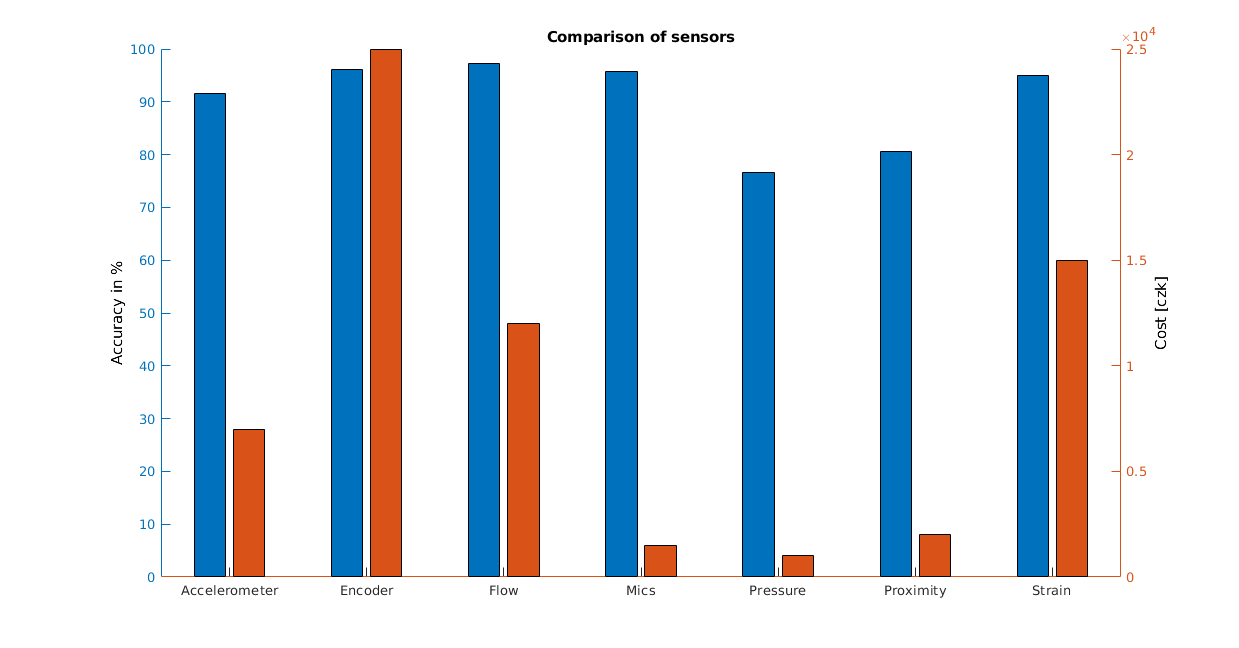
\includegraphics[width=1\textwidth]{sensors_final_bar.png}
    \caption{Comparison of sensors from accuracy/cost perspective}
    \label{fig:sensors_final_bar}
\end{figure}

\begin{table}[h]
    \centering
    \begin{tabular}{|c|c|c|c|c|c|c|c|}
        \hline
        \textbf{Sensor}   & Acc & Encoder & Flow & Mics & Pressure & Proximity & Strain \\
        \hline
        \textbf{Accuracy [\%]} & 91.6 & 96.1 & 97.2 & 95.8 & 76.6 & 80.5 & 95.0 \\
        \hline
        \textbf{Cost [czk]} & 2x 3500 & 25000 & 6000 & 3x 500 & 1000 & 2x 1000 & 15000 \\
        \hline
    \end{tabular}
    \caption{Comparison of sensors from accuracy/cost perspective}
    \label{tab:sensors_final}
\end{table}

\subsection{PdM podle modelu}

Další částí této práce bylo aplikovat modelové metody a použití a
simulační model pro algoritmy prediktivní údržby. Tyto algoritmy
jsou praktické, když je těžké extrahovat užitečné informace pomocí a
metoda založená na signálu. Nebo je to vhodné v některých případech, pokud tomu rozumíme
dynamiku systému a umím využívat některé systémové proměnné jako
indikátory stavu.

Použití metody extrakce funkcí ve formě nelineární
koeficient identifikačního modelu systému, konkrétně s
Hammerstein-Wiener model, nedal spolehlivé výsledky. Extrahované funkce
nemají statistickou závislost a je nemožné předvídat typ poruchy
použitím této metody na naměřených datech z pneumatického pístu jako případ
studie.

Na druhou stranu zbytkový odhad pomocí simulačního modelu
ukázal vynikající výsledky. Měřený signál polohy byl porovnán s
signál ze simulačního modelu v normálním chování. Tento zbytek
signál byl použit ke klasifikaci poruchového stavu a dosažení 99 \% na a
menší datová sada. Ale vzhledem k výsledkům získaným pomocí signálu
Metoda zbytkového odhadu se může zdát zbytečná. V tomhle
konkrétního případu, z praktického hlediska, zlepšení
výsledek o několik procent nepřináší zásadní změny, ale
doba výpočtu se významně zvyšuje.

Byla také ověřena možnost poruch modelování a simulace senzorů
pomocí simulačního modelu. I když je náročné sbírat chyby
data ze snímače v reálných podmínkách mohou být generována data o poruše
od simulačního modelu a dokonce v kombinaci s primární datovou sadou do
vytvořit syntetický datový soubor.

\subsection{RUL}

Jedním z hlavních cílů prediktivní údržby je odhadnout
zbývající životnost. Původní datová sada neobsahuje záznam o
historická data, která ukazují degradační chování.

Běžným problémem při údržbě pneumatických ovladačů je netěsnost
vzduchu z komory, kde je umístěn píst. Tato situace byla
modelované na simulačním modelu a generovaná data byla použita pro RUL
odhad.

Vygenerovaná datová sada obsahuje 25 simulací s různými poruchami
dynamika. Každá simulace zahrnuje jiný počet cyklů v závislosti na tom
na dynamiku selhání, než dojde k selhání systému. Každý cyklus
obsahuje 10sekundové měření odezvy systému. V
experimentu byl jako předmět zájmu vybrán signál toku. Z
signálu toku, byl vypočítán parametr tvarového faktoru a použit jako a
indikátor stavu.

Výsledkem je, že je možné odhadnout zbývající životnost
generovaný datový soubor degradace pomocí modelu zbytkové podobnosti,
model párové podobnosti a model lineární degradace. Předpověď
výsledky jsou uspokojivé.

\subsection{Další vývoj}

Jako další vývoj by bylo vhodné modelovat odhad
parametry systému po částech ke zlepšení výsledků, s důrazem na
vlastnosti škrticích ventilů a tlumičů s úpravami.

Proveďte měření stavu poruchy úniku vzduchu a sbírejte historické údaje
údaje o degradaci skutečného pneumatického pístu. Následně vyhodnotit
dynamika poruchy způsobené únikem vzduchu. Ověřte možnost
odhad zbývající životnosti pomocí snímače průtoku. Může to být
zajímavá případová studie k ověření možnosti použití odhadu RUL
mikrofony. Pokud je výkon dostupných senzorů nedostatečný,
lze provádět měření tlaku v komoře. Tlak v
komora je přímo závislá na úniku vzduchu z komory, jako
uvedené v rovnici \ref{}. Příklad změn tlaku z
simulační model je znázorněn na obrázku \ref{}.
